\adparagraph{Spearman's Footrule}

\begin{figure}[H]
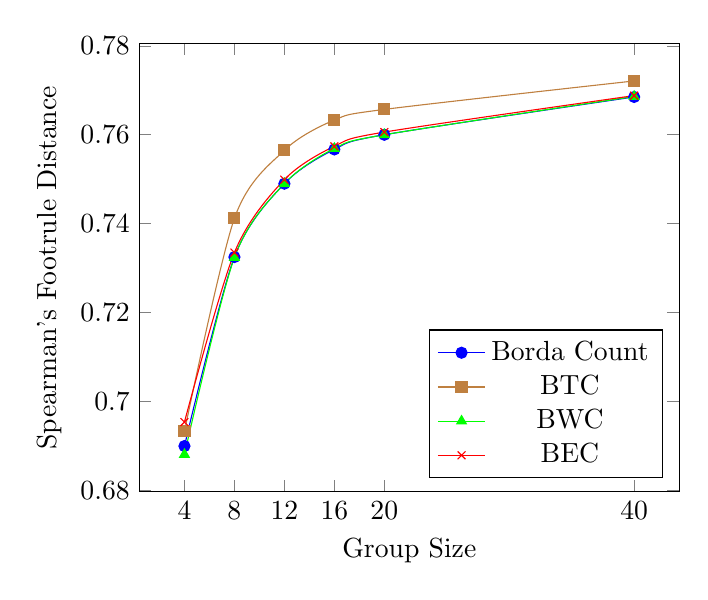
\begin{tikzpicture}
    \begin{axis}[
        xlabel=Group Size,
        ylabel=Spearman's Footrule Distance,
        xtick = {4,8,12,16,20,40},
        legend pos=south east]
    \addplot[smooth,mark=*,blue] plot coordinates {
        (4,0.69)
        (8,0.7325)
        (12,0.749)
        (16,0.7567)
        (20,0.76)
        (40,0.7685)
    };
    \addlegendentry{Borda Count}

 \addplot[smooth,color=brown,mark=square*] plot coordinates {
		(4,0.6933)
		(8,0.7412)
		(12,0.7565)
		(16,0.7633)
		(20,0.7657)
		(40,0.7721)
	};
	\addlegendentry{BTC}
	
	
	\addplot[smooth,color=green,mark=triangle*] plot coordinates {
		(4,0.6881)
		(8,0.7324)
		(12,0.749)
		(16,0.7569)
		(20,0.76)
		(40,0.7686)
	};
	\addlegendentry{BWC}
	
	
	\addplot[smooth,color=red,mark=x] plot coordinates {
		(4,0.6954)
		(8,0.7335)
		(12,0.7499)
		(16,0.7574)
		(20,0.7606)
		(40,0.7688)
	};
	\addlegendentry{BEC}
    
    \end{axis}
\end{tikzpicture}
\caption{Results on Spearman's Footrule distance test for Borda Count extensions}
\end{figure}